\documentclass[../main/thesis.tex]{subfiles}
\begin{document}
%\appendixpagenumbering
%\chapter{Appendix}
%\addcontentsline{toc}{chapter}{Appendix}
%\appendixpagenumbering
%\appendix
%\section{PCB for detector connection}
%\appendixpagenumbering
\chapter{Detector Interface PCB}
\label{a-pcb}

A \gls{PCB} was needed to connect the detector to the characterization equipment, as the detector pads are too small for any other connection than wire-bonding. This \gls{PCB} could simply have consisted of wire-bonding pads going to connectors for cables, but it was decided to make a more multi-purpose board to make it simple to try different setups. The board was made so that it is possible to connect the substrate, the guard rings, and the p+ rings individually to ground or external bias. It is also possible to read out the guard rings of the cells. Each channel can also be connected to a bias filter for removal of high frequency noise. The n+ core readout channel was designed to add as little capacitance as possible. LEMO connectors were chosen to connect to the readout system as they are well shielded and much used at \gls{ift}. The exposed metal is coated with electroless nickel immersion gold (ENIG) to provide better contact for wire-bonding. A mistake was done with the \gls{PCB} design in that solder mask where the detector is mounted was forgotten. This has no consequences for the 3DMiMic detector, since there is an insulating layer between the bulk and the support wafer. The solder resist can be scratched off if the \gls{PCB} is to be used for a different detector. A picture of the \gls{PCB} can be seen in figure \ref{fig-pcb-pic} and the layout can be seen in figure \ref{fig-pcb}. 

\begin{figure}[h]
	\centering
	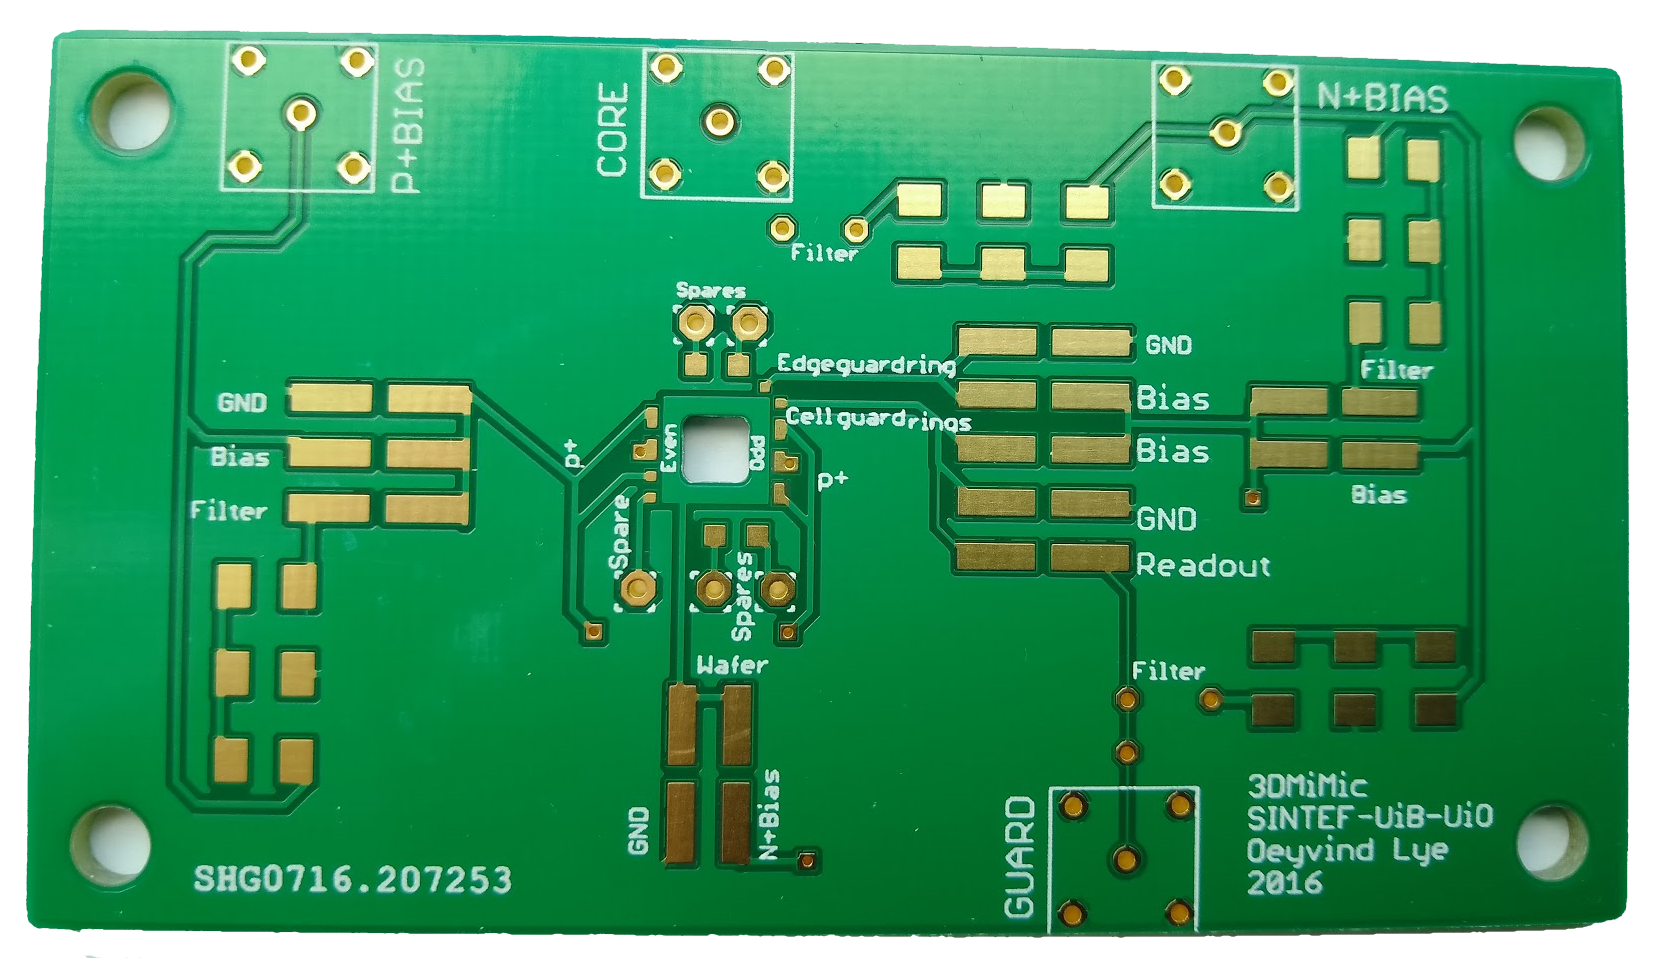
\includegraphics[width=0.95\textwidth]{pcb-pic.png}
	\caption{Top side of PCB.}
	\label{fig-pcb-pic} 
\end{figure}

\begin{figure}%[h]
	\centering
	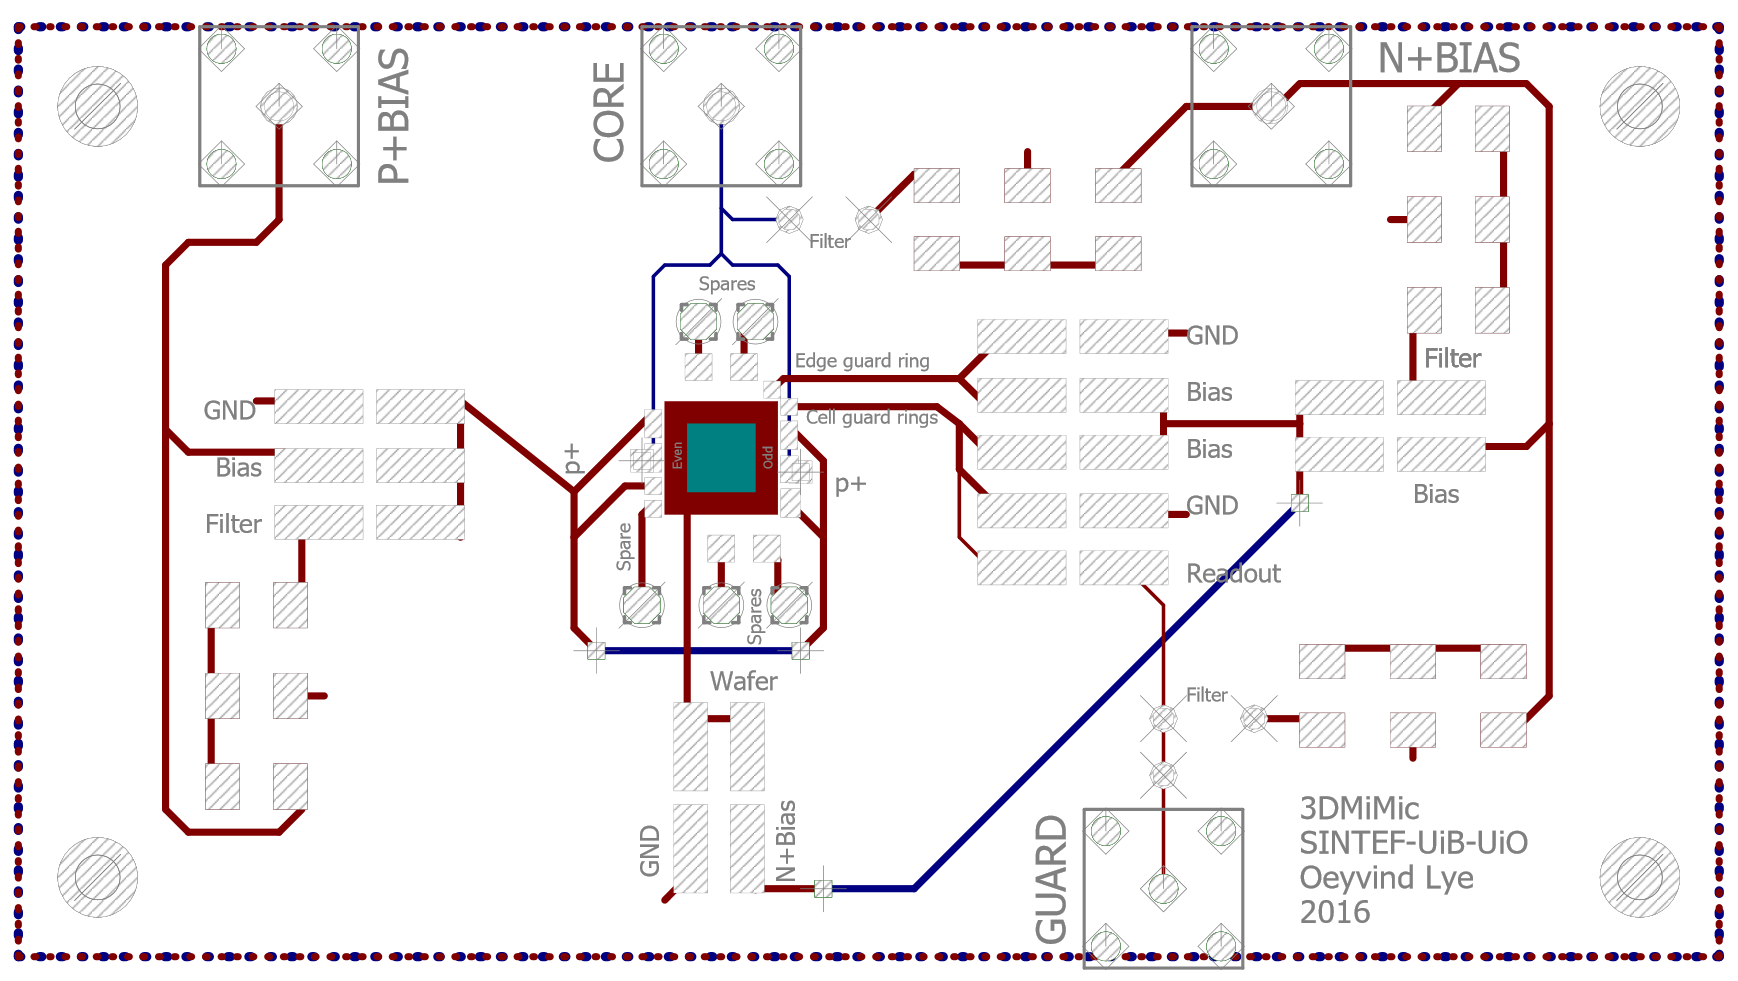
\includegraphics[angle=270,width=0.8\textwidth]{pcb.png}
	\caption{PCB layout. Ground planes not shown.}
	\label{fig-pcb} 
\end{figure}

After the design had been produced, it was again considered to read out the two sides of the detector separately, instead of in one signal. On the \gls{PCB}, this can be solved by wire-bonding one of the sides to one of the spare pads and connecting this to the through-hole by the GUARD connector with a wire. To avoid extra capacitance, the wires leading to the unused surface-mounting pads can be cut with a knife. If cutting the wires after the detector has been mounted, try to protect the detector from flying debris. A new layout for two channel readout has been designed, and can be produced when needed. 

\gls{uib} uses an X-Y table to position detectors during beam tests. This can move the detector in two dimensions with small, controlled steps. A mount was designed that can be used to connect the PCB to the X-Y table, see figure \ref{fig-xytable-picture}. 

\begin{figure}[h]
	\centering
	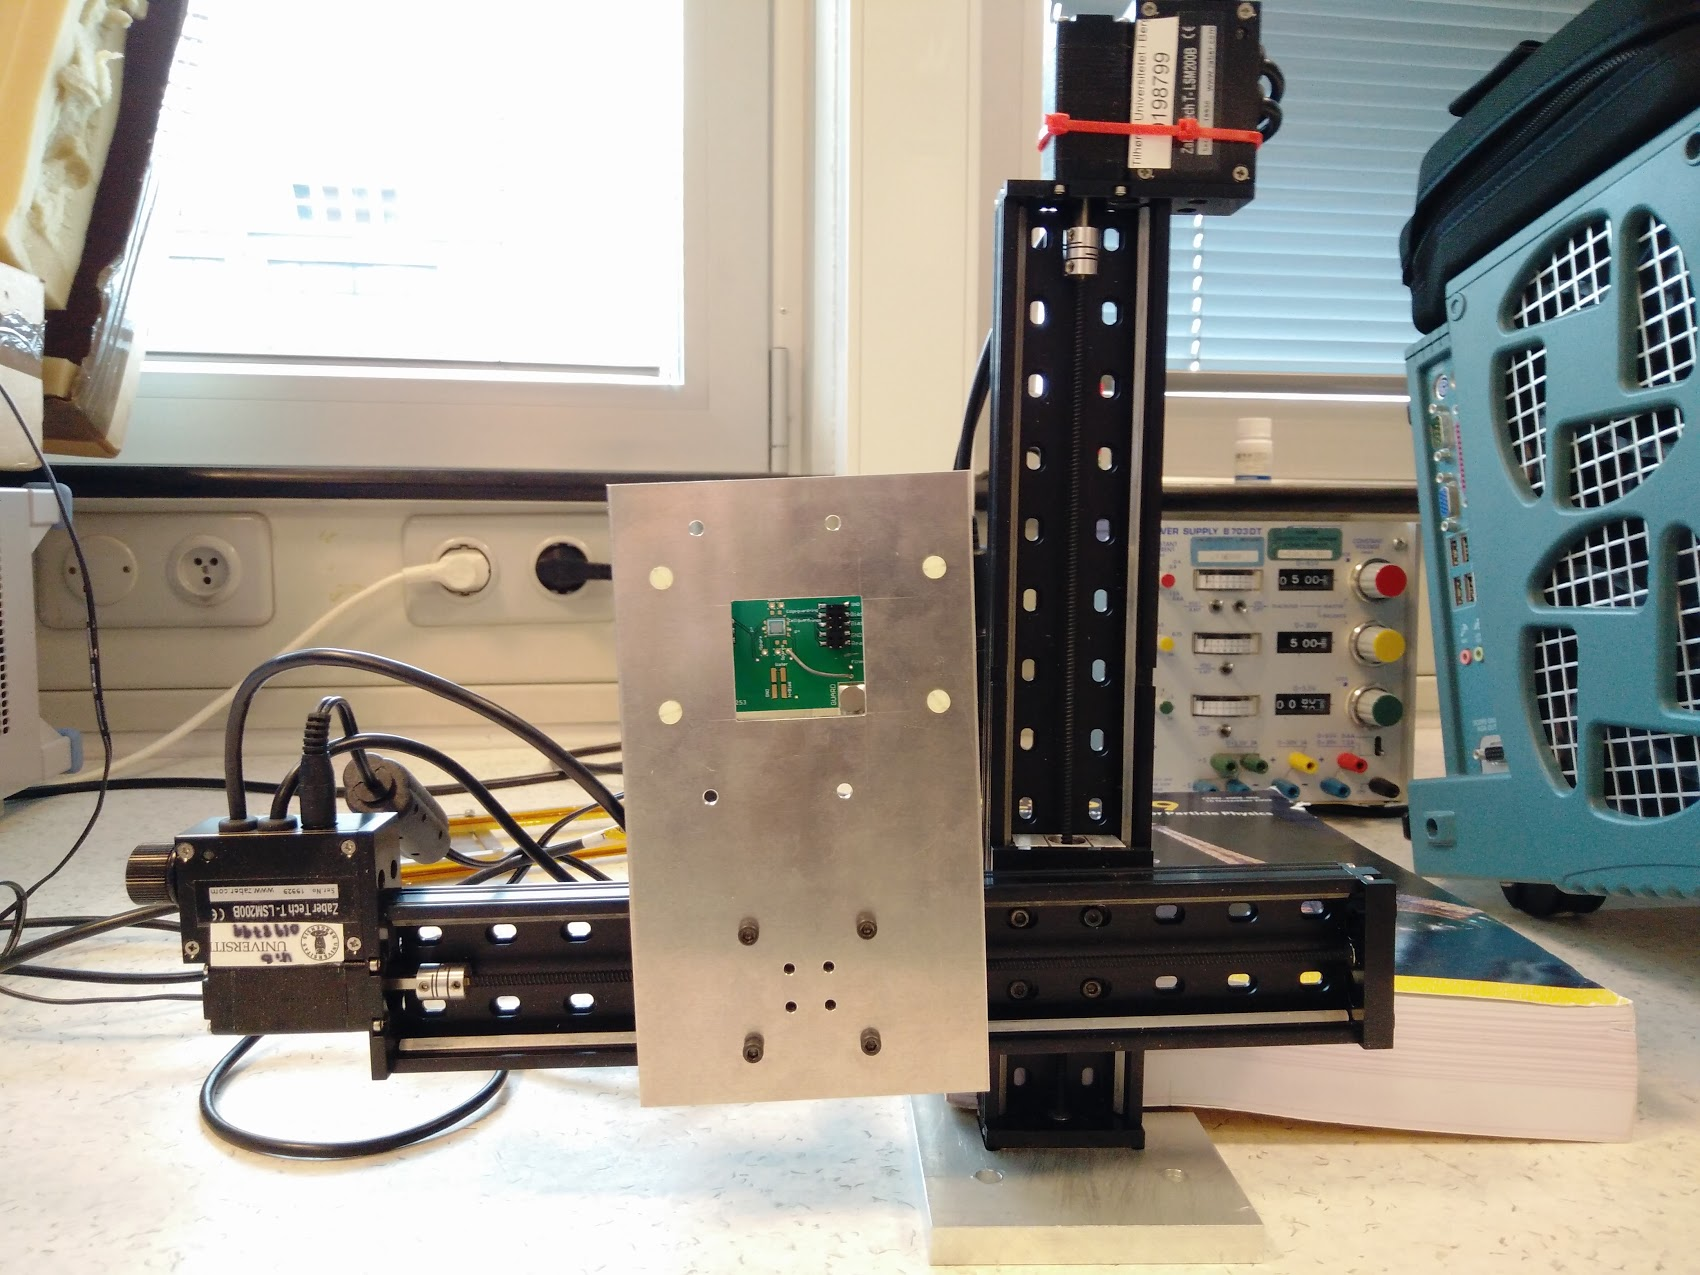
\includegraphics[width=\textwidth]{xytable.jpg}
	\caption{3DMiMic PCB mounted on X-Y table.}
	\label{fig-xytable-picture}
\end{figure} 

Figures \ref{fig-wire-1-g} to \ref{fig-wire-2} show how wire-bonding should be performed for different detectors and readout schemes. Figures \ref{fig-wiring-1-g} to \ref{fig-wiring-2} show where external wires (red) should be soldered, and where PCB lanes should be cut (black). Dotted line for optional wires not necessary for detector operation.

\begin{figure}%[h]
	\centering
	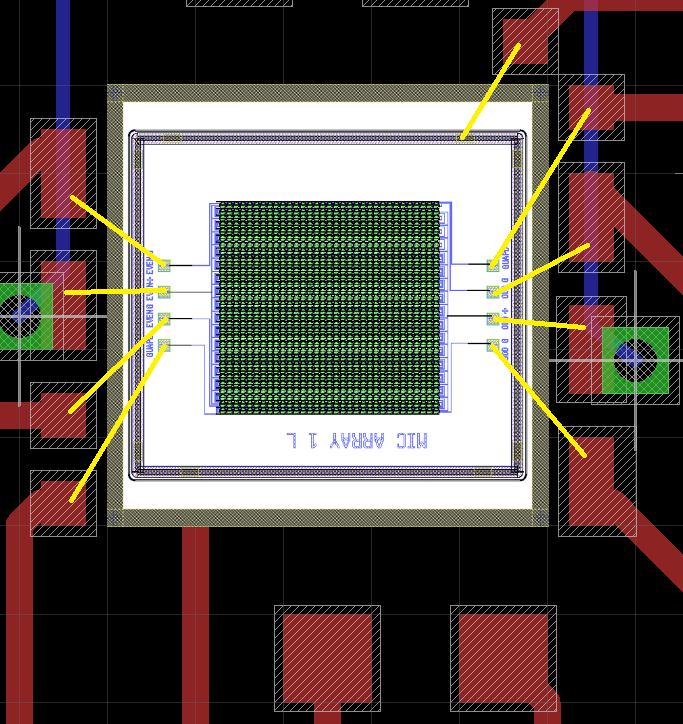
\includegraphics[width=0.6\textwidth]{w_single_channel.png}
	\caption{Wirebonding for single channel readout on a detector with n+ guard rings.}
	\label{fig-wire-1-g} 
\end{figure}

\begin{figure}%[h]
	\centering
	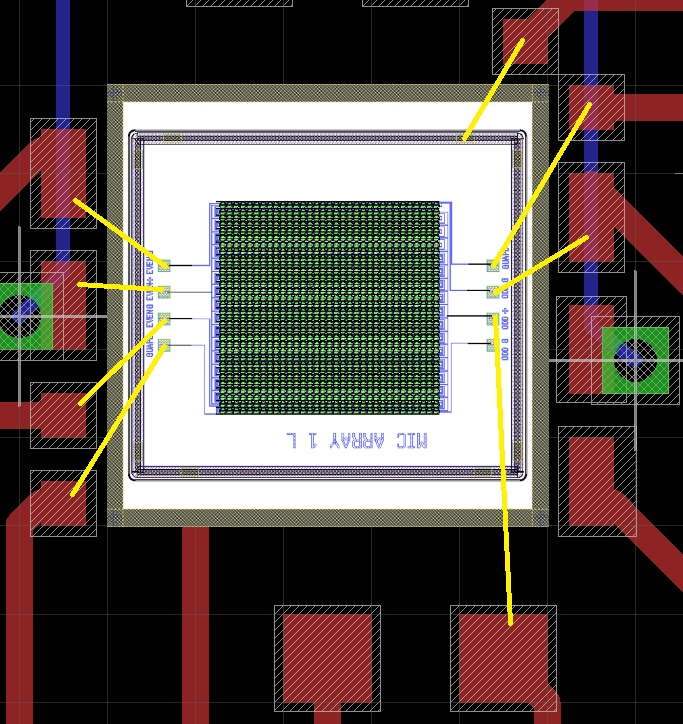
\includegraphics[width=0.6\textwidth]{w_two_channel_guard.png}
	\caption{Wirebonding for two channel readout on a detector with n+ guard rings.}
	\label{fig-wire-2-g} 
\end{figure}

\begin{figure}%[h]
	\centering
	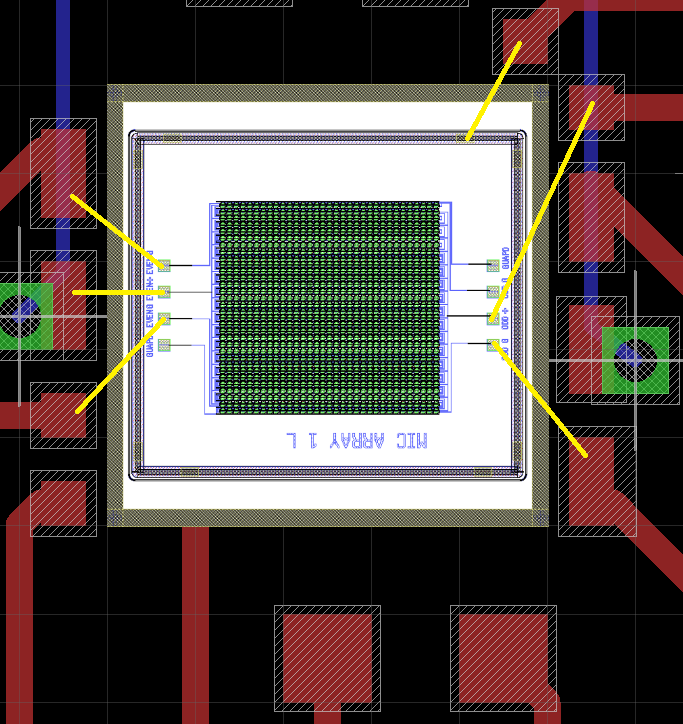
\includegraphics[width=0.6\textwidth]{w_two_channel_no_guard.png}
	\caption{Wirebonding for two channel readout on a detector without n+ guard rings.}
	\label{fig-wire-2} 
\end{figure}

\begin{figure}%[h]
	\centering
	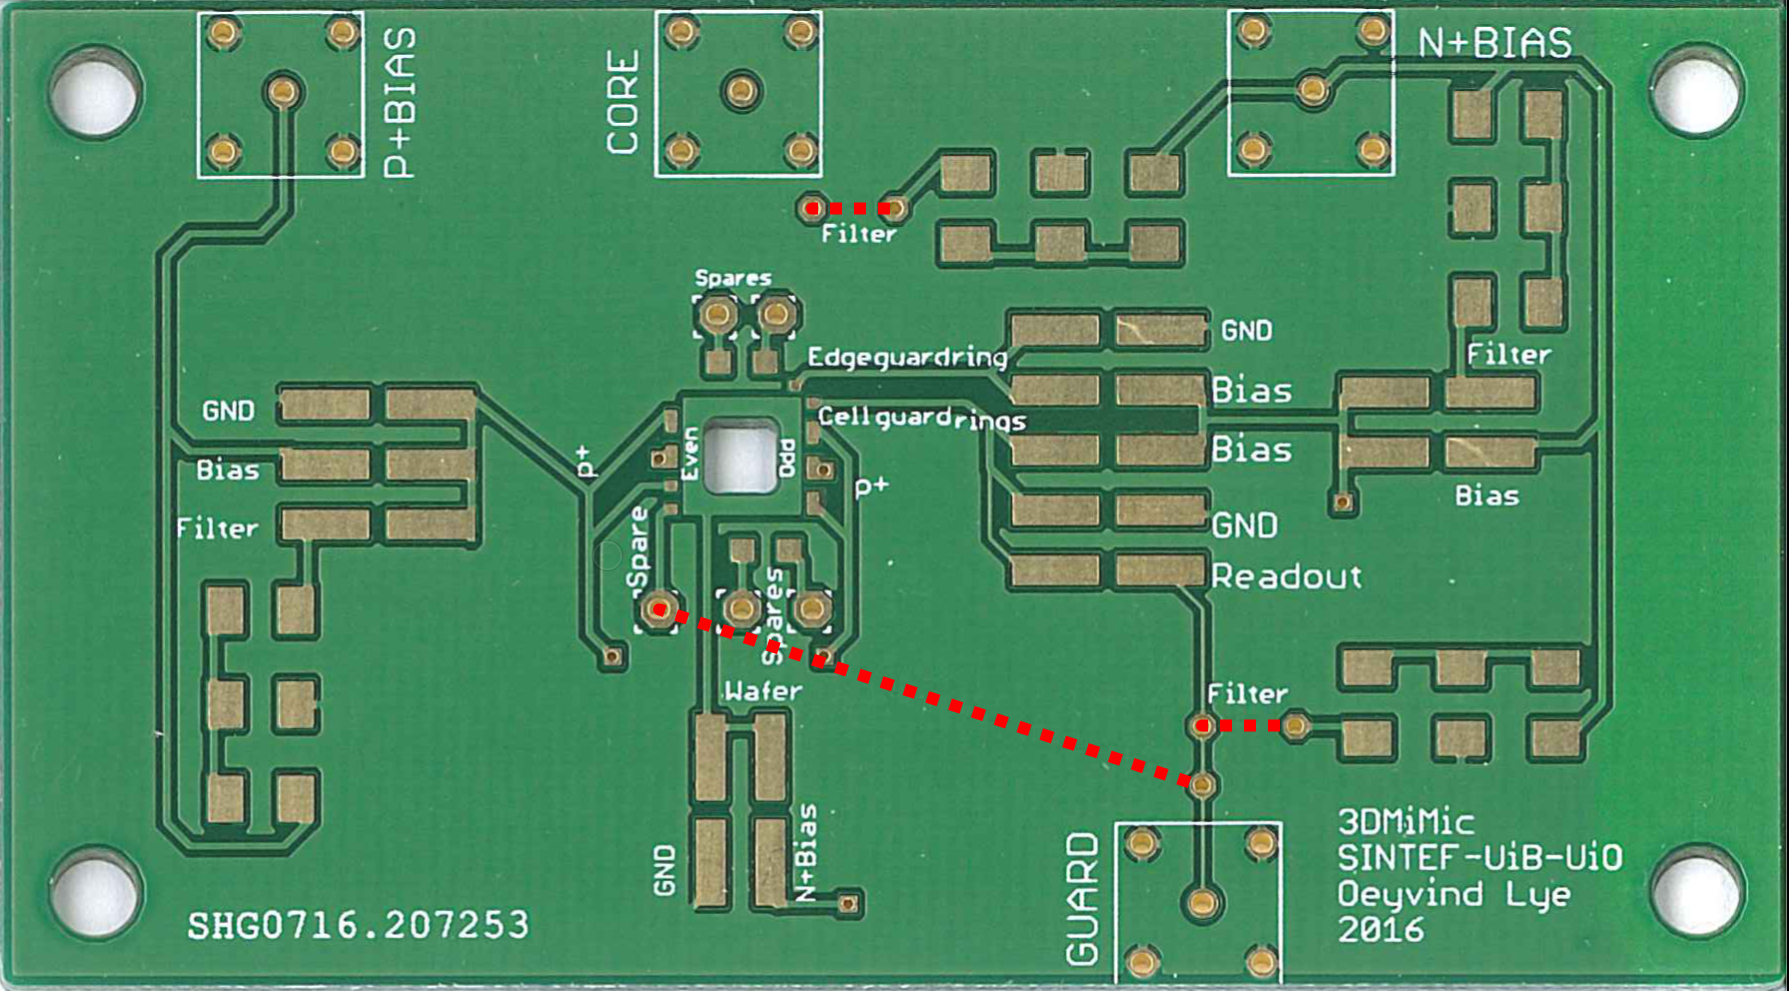
\includegraphics[width=0.8\textwidth]{pcb-pic-single-channel.png}
	\caption{Wiring for single channel readout on a detector with n+ guard rings.}
	\label{fig-wiring-1-g} 
\end{figure}

\begin{figure}%[h]
	\centering
	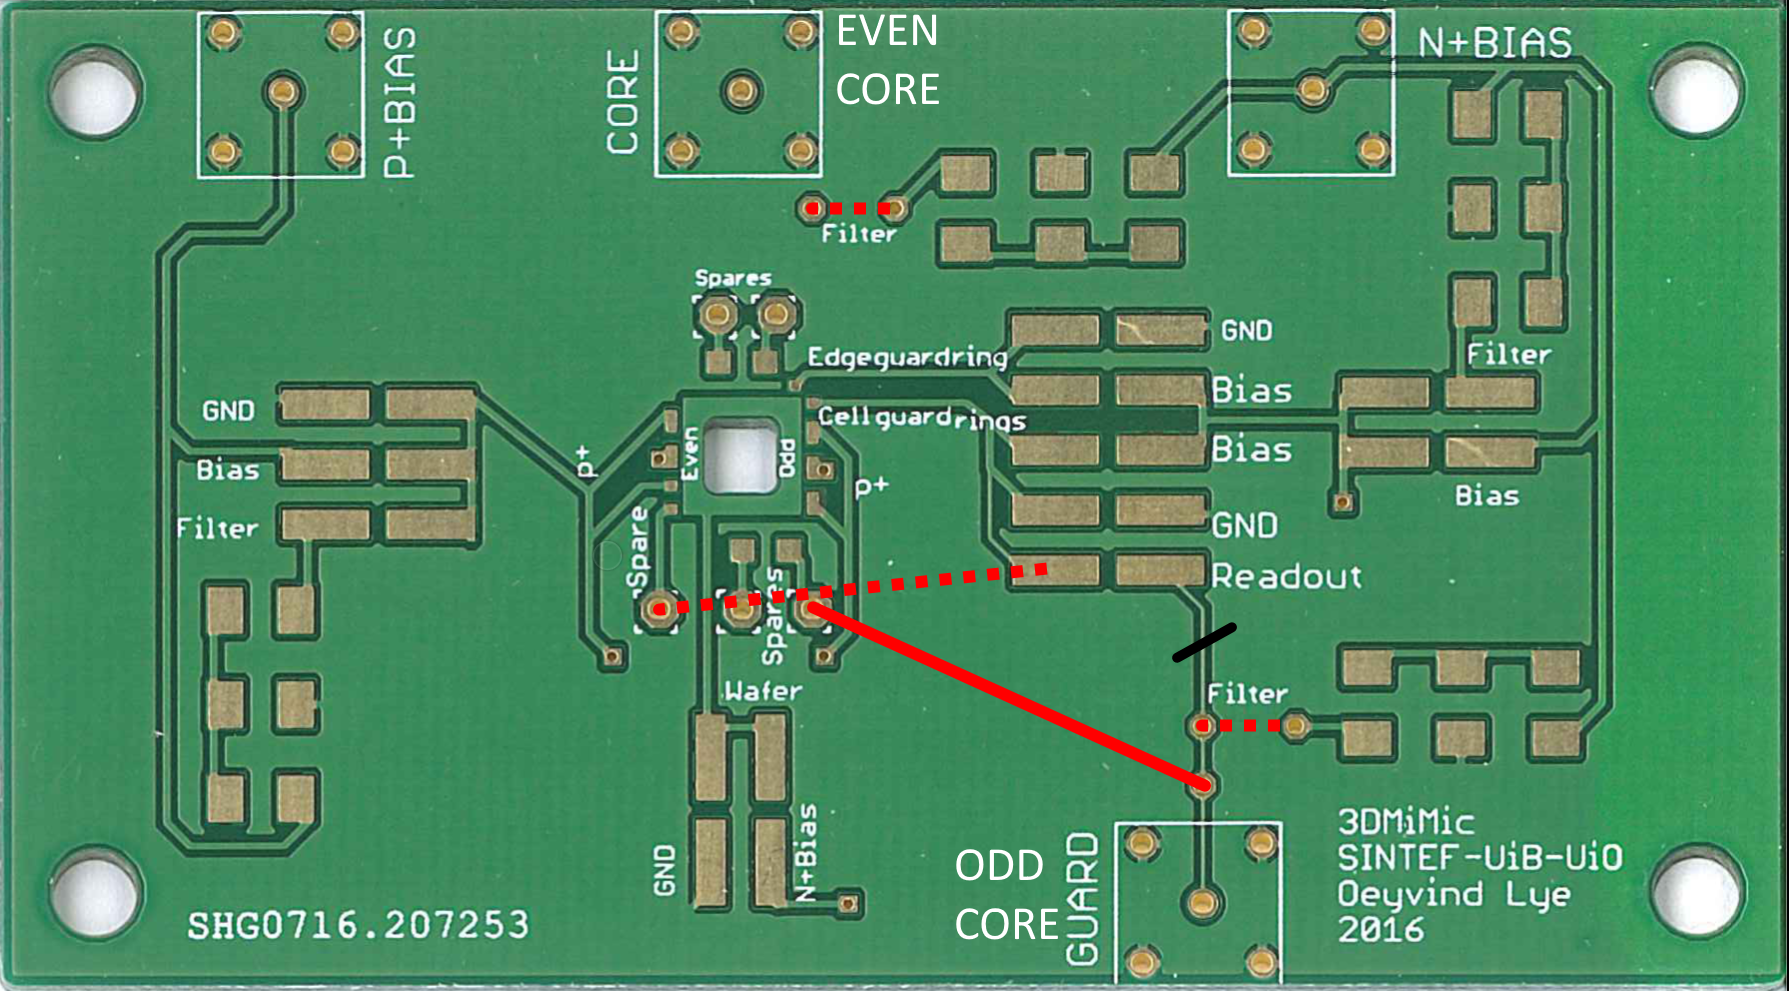
\includegraphics[width=0.8\textwidth]{pcb-pic-two-channel-guard.png}
	\caption{Wiring for two channel readout on a detector with n+ guard rings.}
	\label{fig-wiring-2-g} 
\end{figure}

\begin{figure}%[h]
	\centering
	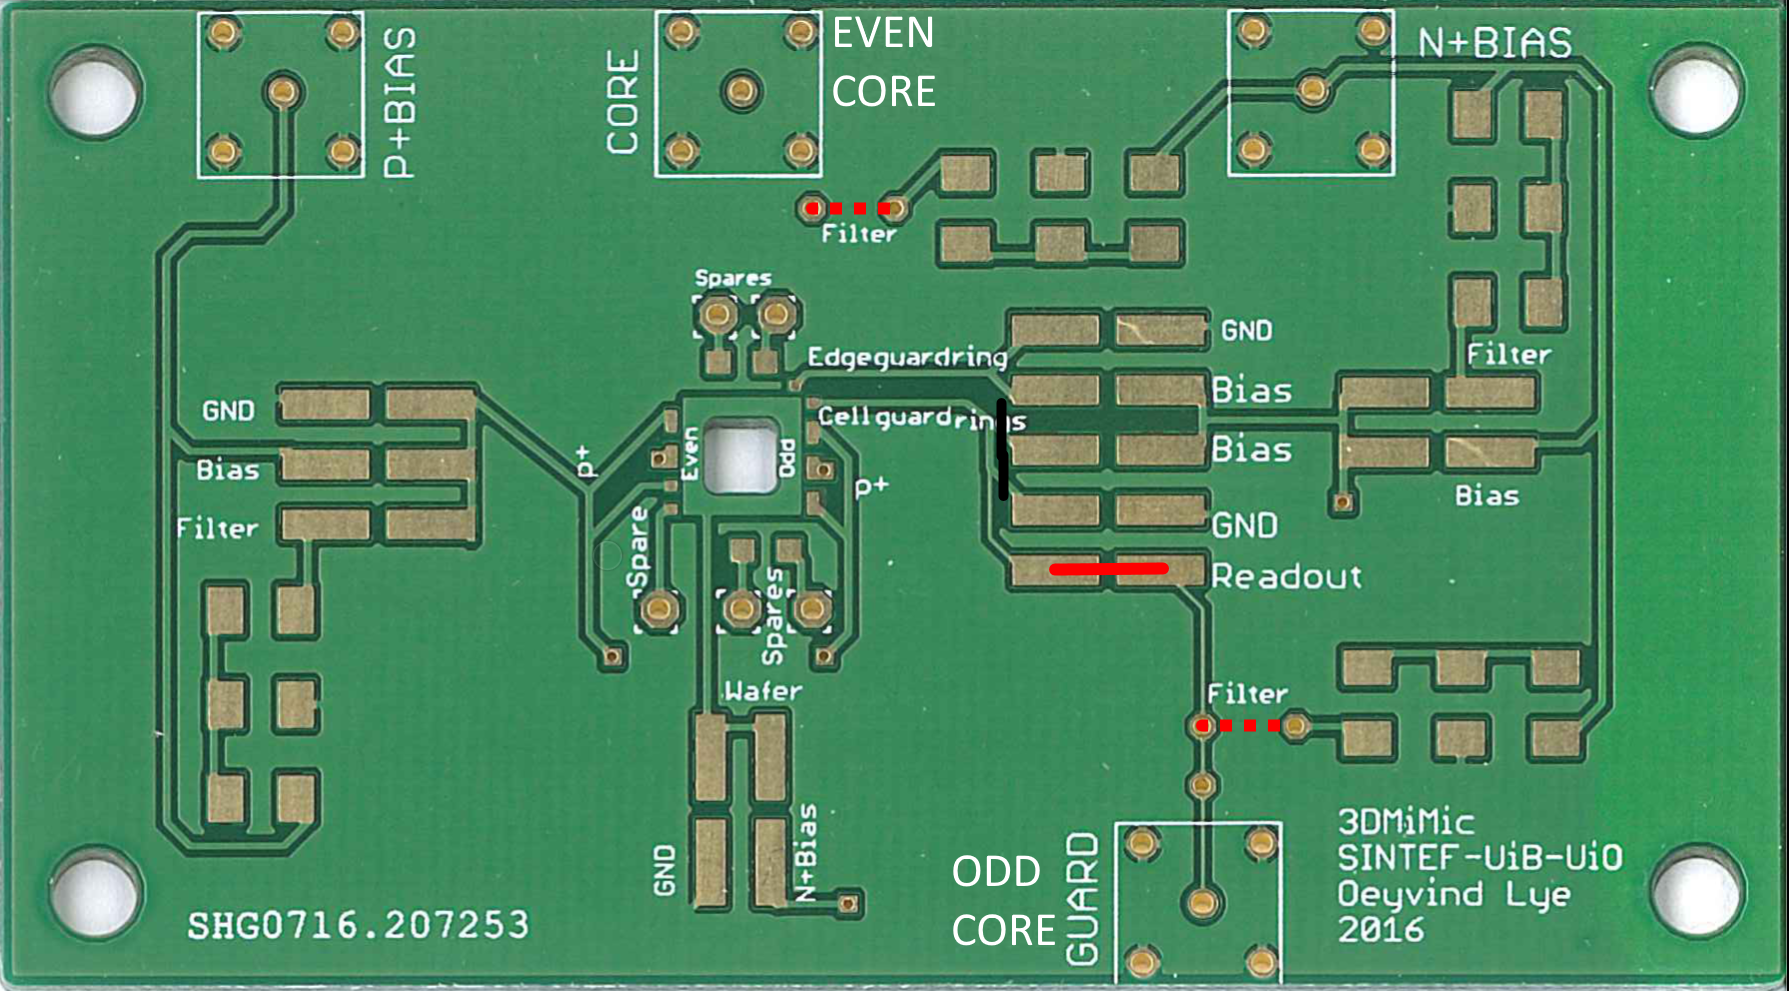
\includegraphics[width=0.8\textwidth]{pcb-pic-two-channel-no-guard.png}
	\caption{Wiring for two channel readout on a detector without n+ guard rings.}
	\label{fig-wiring-2} 
\end{figure}

A new version of the PCB layout will be designed an published to UiB's Macaos account shortly after this thesis is delivered. It will be designed specifically for two channel readout and feature some other minor improvements. This includes adding solder mask under the detector, adding option to mount the detector on the other side of the PCB, moving spare pads closer to the detector, and adding text for the connectors on the other side of the PCB. 

\comm{
New version:
two channel readout
solder mask detektor
detector both sides
spares closer
text both sides}

\end{document}